\chapter{Avaliação quantitativa}\label{chap:avaliacao}

O objetivo deste capítulo é descrever as avaliações utilizadas na solução proposta. A avaliação tem como objetivo determinar a performance e acurácia do mecanismo de descoberta, conexão e desconexão de \smartobjs{}.

A avaliação será realizada por meio de experimentos, onde a performance será avaliada através da contagem de tempo desde que o \mhub{} efetivamente descobre um objeto até o momento em que a aplicação é informada sobre este evento. A acurácia da solução consistirá na verificação de quantas operações de conexão, desconexão e descoberta geraram eventos correspondentes para a aplicação.

\section{Descrição dos experimentos}

Foi desenvolvido um aplicativo android utilizando o \mhubcddl{} onde o \smartphone{} permanece ativamente procurando e, quando possível, se conectando a \smartobjs{} no ambiente. O aplicativo é responsável por registrar a ocorrencia de interações com \smartobjs{}, juntamente com os \timestamps{} de cada um desses eventos. Os experimentos foram realizados no âmbito de dois cenários de uso descritos a seguir.

Os cenários de uso foram simulados com a tecnologia \fakesensor{} para gerar os eventos no \stwopa{}.

\subsection{Cenário de uso 1}

Este cenário de uso consiste em uma casa onde cada cômodo é equipado com um \beacon{} \ble{}, calibrado de forma que o sinal emitido não possa ser detectado fora do cômodo e configurado para emitir 10 anúncios por segundo. Uma pessoa carregando o \smartphone{} é instruida a conduzir as atividades do dia a dia normalmente, e o aplicativo detecta em qual região da casa o indivíduo se encontra.

Ao entrar em um cômodo, o \beacon{} será encontrado pelo \mhubcddl{}, gerando um evento de descoberta no \stwopa{} que deverá ser propagado para a aplicação.

\subsection{Cenário de uso 2}

Consiste em uma casa que possui um sistema multimídia na sala de estar, onde o conteúdo da televisão se adapta de acordo com os usuários que estão presentes na sala de estar, e a interação com as aplicações da televisão digital acontece através do \smartphone{}.

Ao entrar na sala de estar o sistema multimídia é encontrado e em seguida a conexão é estabelecida. Quando o usuário sai da sala de estar a conexão é desfeita. É medido o tempo de propagação de todos os eventos de descoberta, conexão e desconexão gerados no \stwopa{} para a aplicação.

\section{Descrição dos dados}

Ambos os cenários de uso foram simulados, os dados utilizados para a simulação foram obtidos do \dataset{} disponibilizado por \citeonline{byrne2018residential}\footnote{O \dataset{} pode ser obtido em \cite{byrne2019dataset}}. Neste trabalho os autores instruiram que participantes conduzissem suas rotinas diárias em casa, enquanto sua localização na residência era monitorada.

O chão dos cômodos das casas foi marcado com etiquetas, as etiqueta são uma imagem binária que codifica um número inteiro, e este, único para cada uma das etiquetas. Os participantes são equipados com uma câmera na região do torso que aponta em direção ao chão, detectando e interpretando qual etiqueta está visível no momento, e deste modo, identificando em qual cômodo o participante se encontra.

Utilizou-se os dados do experimento denominado de ``\texttt{living\_2}'' da casa referida como ``\texttt{Residence D}''. Os dados deste experimento consistem de 58 minutos de monitoramento de um indivíduo realizando suas atividades cotidianas em uma casa de 10 cômodos. Os dados possuem uma resolução média de aproximadamente 11 medições por segundo. 

Para o cenário de uso 2 utilizou-se o cômodo ``\texttt{living\_area\_A}'' como a sala de estar onde o sistema multimídia se localiza. As informações referentes a quantidade de vezes que o participante entra em cada cômodo estão sumarizadas na \autoref{fig:dataset-histogram}.

\begin{figure}[htb]
	
	\begin{center}
		
		\caption{\label{fig:dataset-histogram}Frequência de entrada por cômodo}
		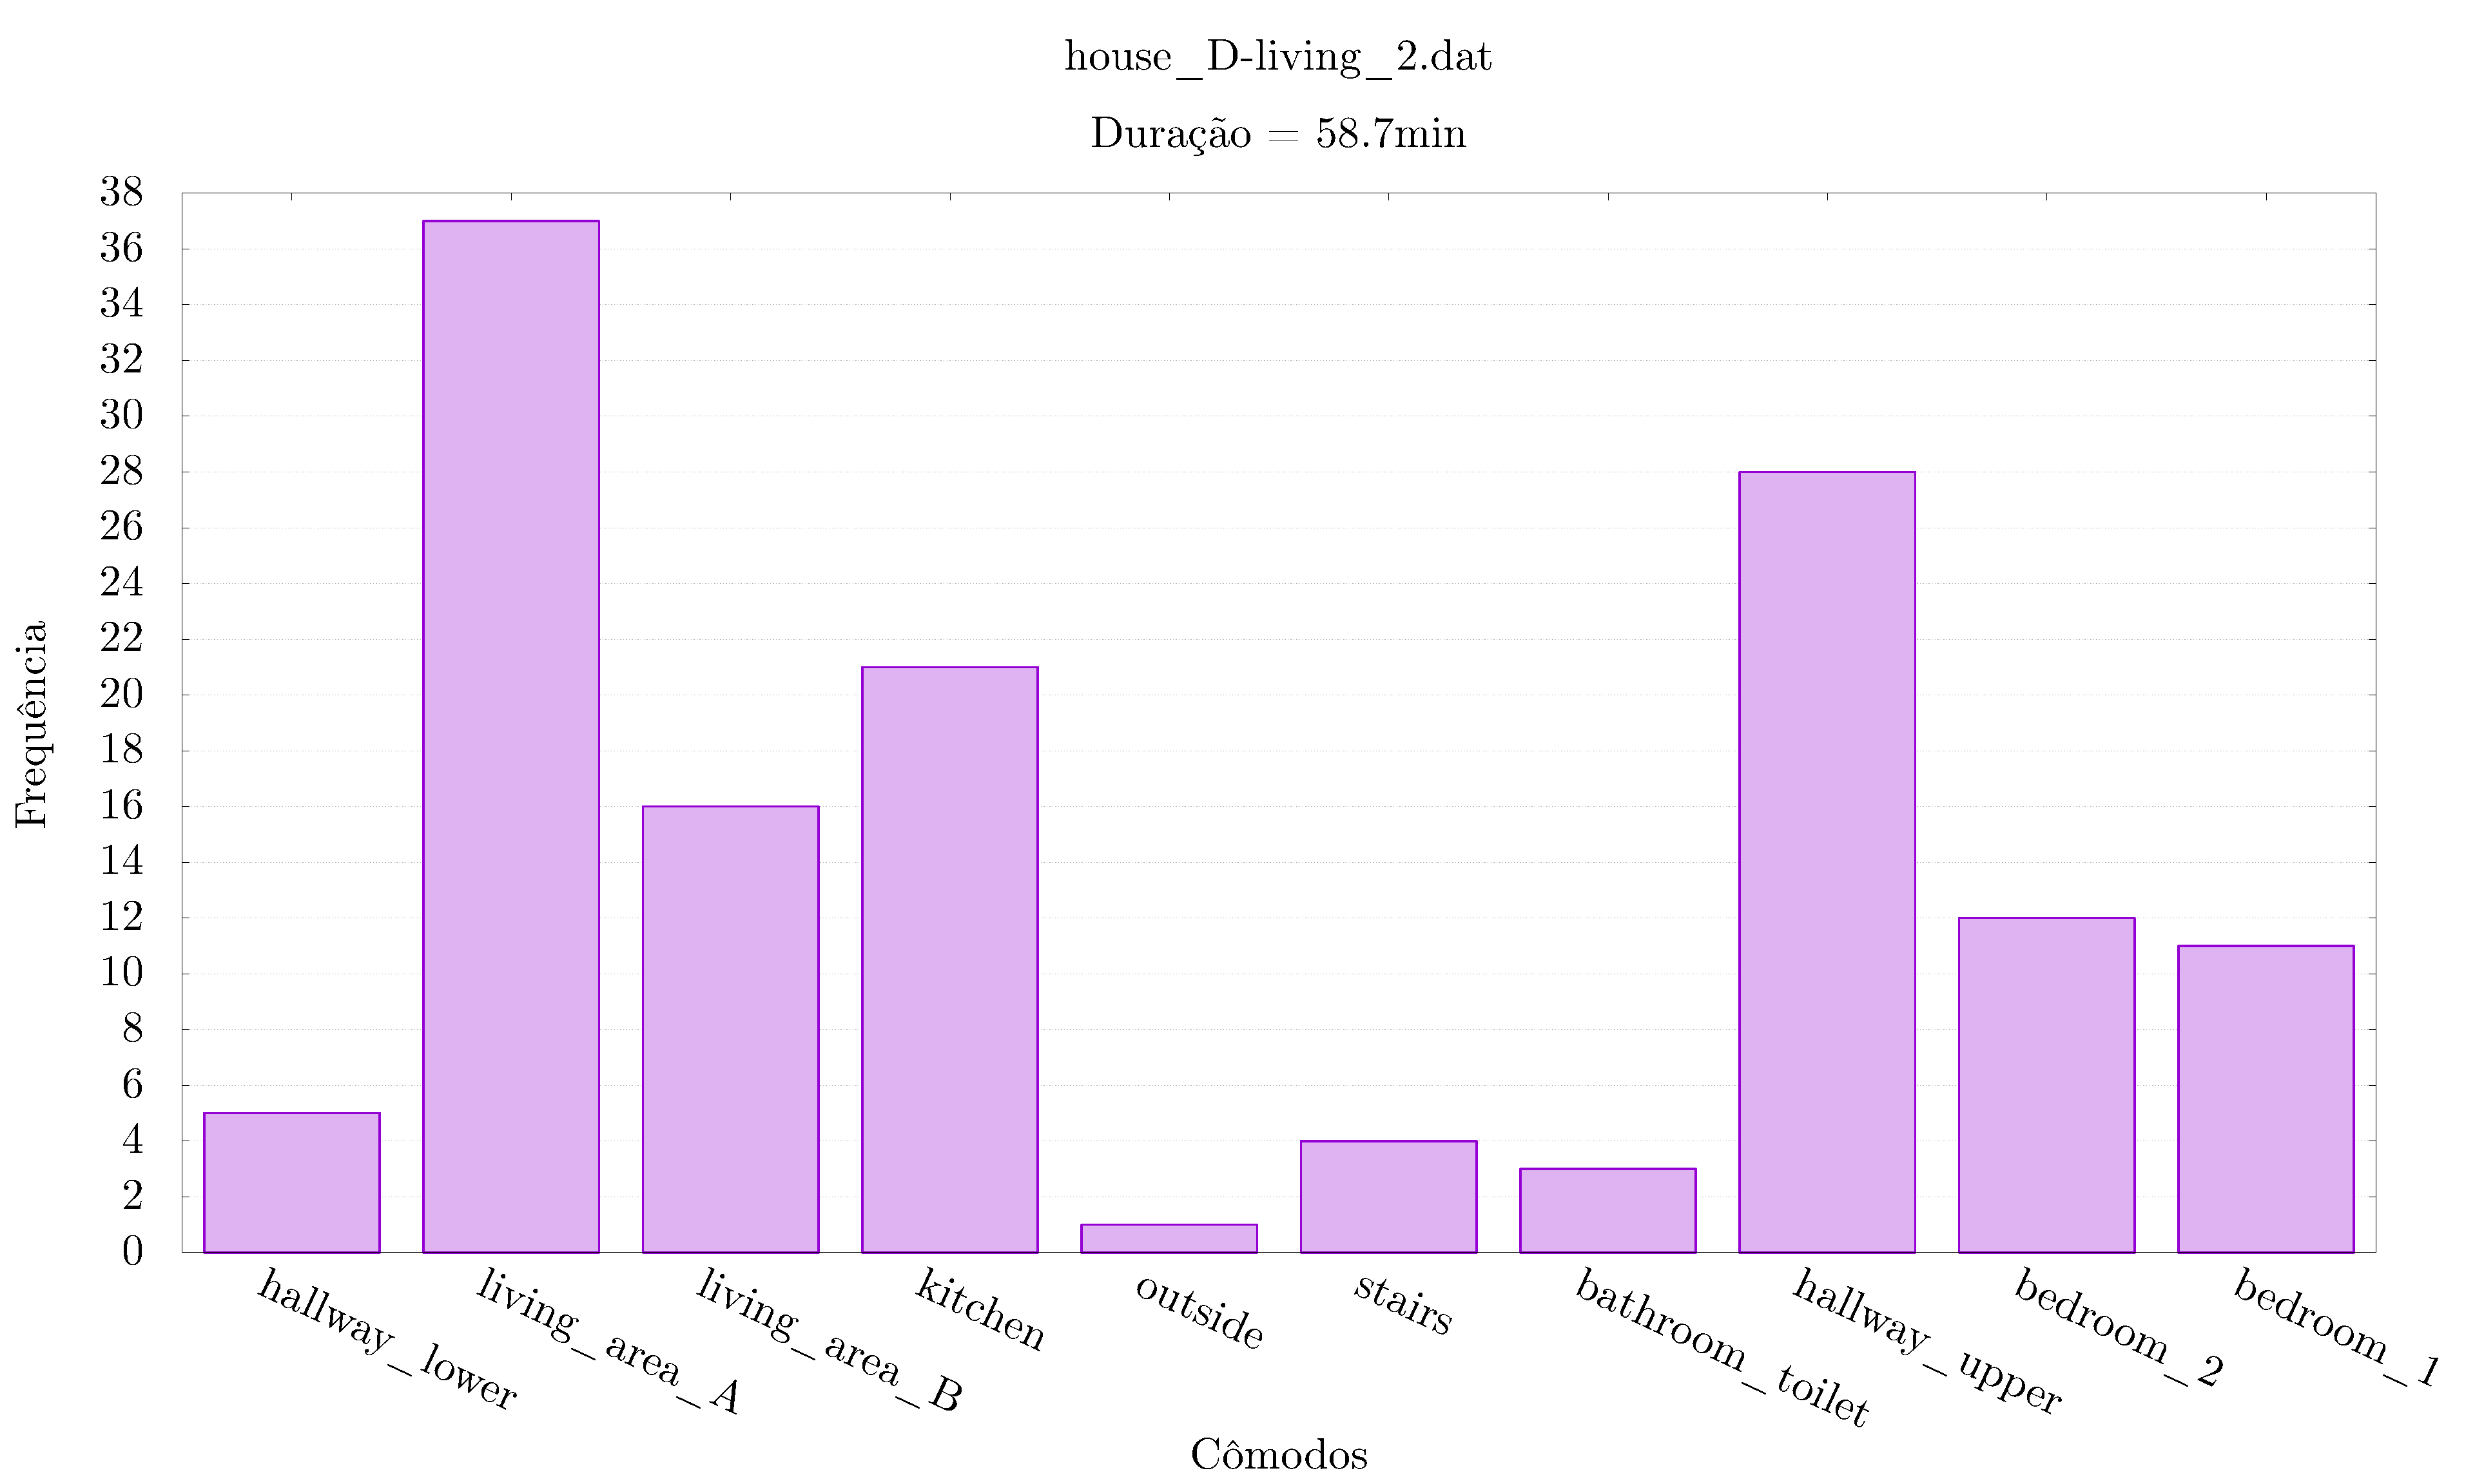
\includegraphics[scale=0.246]{img/dataset-histogram}
		\fonte{\autoriapropria{}}
		
	\end{center}

\end{figure}

\section{Métricas}

Para o cenário de uso 1, o aplicativo detecta um anúncio a cada 0.1 segundo em que o participante permanece em um cômodo. Cada anúncio detectado corresponde a um evento de descoberta no \stwopa{}, este evento deve então ser propagado até a aplicação, a aplicação permanece constantemente anotando os \timestamps{} de cada evento e calculando o tempo de propagação, sendo assim possível obter uma métrica de desempenho. Para avaliar a acurácia é realizada uma comparação entre quantos eventos foram gerados e quantas notificações foram entregues à aplicação.

Para o cenário de uso 2, a todo momento em que o participante entra na sala de estar acontece interações entre o aplicativo e o sistema multimídia, essas interações são compostas de um evento de descoberta, seguido por um evento de conexão. Ao sair do quarto um evento de desconexão é também gerado. 

As avaliaçãos de desempenho e acurácia deste cenário de uso são análogas às do cenário de uso 1, com a exceção de que eventos de conexão e desconexão também fazem partes das medições.

A \autoref{tab:expected-results-1} e a \autoref{tab:expected-results-2} mostram os resultados esperados de ambos os cenários de uso. Estes valores serão utilizados para a análise de acurácia da solução.

\begin{table}[htb]
	\begin{center}
		\IBGEtab{
			\caption{Resultados esperados do cenário de uso 1}
			\label{tab:expected-results-1}
		}{
			\begin{tabular}{lc}
				\toprule
				& \textbf{Cenário de uso 1 (Esperado)}	    \\
				\midrule \midrule
				\textbf{Eventos de descoberta}	& 34814	    \\
				\textbf{Eventos de conexão}	& 0	    \\
				\textbf{Eventos de desconexão}	& 0	    \\
				\bottomrule
			\end{tabular}
		}{
			\fonte{\autoriapropria}
		}
	\end{center}
\end{table}

\begin{table}[htb]
	\begin{center}
		\IBGEtab{
			\caption{Resultados esperados do cenário de uso 2}
			\label{tab:expected-results-2}
		}{
			\begin{tabular}{lc}
				\toprule
				& \textbf{Cenário de uso 2 (Esperado)}	\\
				\midrule \midrule
				\textbf{Eventos de descoberta}	& 140	\\
				\textbf{Eventos de conexão}	& 140	\\
				\textbf{Eventos de desconexão}	& 139	\\
				\bottomrule
			\end{tabular}
		}{
			\fonte{\autoriapropria}
		}
	\end{center}
\end{table}



